\documentclass[12pt, a4paper]{article}

\usepackage{fontspec}
\setmainfont{FreeSerif}
\setsansfont{FreeSans}
\setmonofont{FreeMono}

\usepackage{amsmath, amsthm, amssymb}
\usepackage{mathtools}
\usepackage{enumitem}
\usepackage{microtype}
\usepackage{geometry}
\usepackage{hyperref}
\usepackage{xcolor}
\usepackage{tikz}
\usetikzlibrary{arrows.meta, positioning}

\tolerance=1000
\emergencystretch=2em

\geometry{
  a4paper,
  top=2.5cm, bottom=2.5cm,
  left=3cm, right=3cm
}

\hypersetup{
  colorlinks=true,
  linkcolor=blue!60!black,
  urlcolor=blue!60!black
}

% ---------- theorem environments ----------
\theoremstyle{plain}
\newtheorem{theorem}{Theorem}
\newtheorem{lemma}[theorem]{Lemma}
\newtheorem{corollary}[theorem]{Corollary}

\theoremstyle{definition}
\newtheorem{definition}[theorem]{Definition}
\newtheorem{remark}[theorem]{Remark}

% ---------- notation shortcuts ----------
\newcommand{\proves}{\vdash}
\renewcommand{\models}{\vDash}
\newcommand{\Lang}{\mathcal{L}}
\newcommand{\Lw}{\mathcal{L}_\omega}
\newcommand{\Struct}{\mathfrak{M}}
\newcommand{\tuple}[1]{\langle #1 \rangle}
\newcommand{\N}{\mathbb{N}}

% ---------- document ----------
\begin{document}

\title{\textbf{G\"odel's Completeness Theorem\\
for First-Order Predicate Calculus}}
\author{}
\date{}
\maketitle
\tableofcontents
\bigskip

% ==============================================
\section{Statement of the Problem}
% ==============================================

Fix a first-order language $\Lang$ with a \emph{finite signature}:
a finite set of predicate symbols $P_1,\ldots,P_k$,
function symbols $f_1,\ldots,f_m$, and constants $a_1,\ldots,a_n$.
Let $\Lang^0$ denote the set of all \emph{closed} formulas (sentences) of the language~$\Lang$.

\begin{theorem}[G\"odel, 1930]\label{thm:completeness}
Let $\Gamma \subseteq \Lang^0$ and $\varphi \in \Lang^0$. Then
\[
  \Gamma \models \varphi \iff \Gamma \proves \varphi.
\]
\end{theorem}

The direction $(\Leftarrow)$ --- \emph{soundness} --- is proved by a standard induction
on derivations, and we omit it. The substantial content of the theorem is the
direction $(\Rightarrow)$, \emph{completeness}, to which this text is devoted.

Contrapositively, completeness is equivalent to the following statement:

\begin{lemma}[Model Existence]\label{lem:model-existence}
Every consistent set $\Gamma \subseteq \Lang^0$ is satisfiable,
i.e., there exists an $\Lang$-structure $\Struct$ such that $\Struct \models \varphi$
for all $\varphi \in \Gamma$.
\end{lemma}

The rest of this text is devoted to the proof of this lemma.

% ==============================================
\section{Preliminaries}
% ==============================================

\subsection{Structures and Truth}

\begin{definition}
An \emph{$\Lang$-structure} $\Struct = \tuple{M, \{P_i^{\Struct}\}, \{f_j^{\Struct}\}, \{a_l^{\Struct}\}}$
consists of:
\begin{itemize}
  \item a nonempty set $M$ --- the \emph{carrier};
  \item an interpretation of each predicate symbol $P_i$ as a relation
        $P_i^{\Struct} \subseteq M^{\text{ar}(P_i)}$;
  \item an interpretation of each function symbol $f_j$ as a function
        $f_j^{\Struct}\colon M^{\text{ar}(f_j)} \to M$;
  \item an interpretation of each constant $a_l$ as an element $a_l^{\Struct} \in M$.
\end{itemize}
\end{definition}

The truth of a closed formula $\varphi$ in a structure $\Struct$
(notation: $\Struct \models \varphi$) is defined by the standard
recursion on the construction of~$\varphi$:
\begin{itemize}
  \item $\Struct \models P_i(t_1,\ldots,t_k)$ if
        $\tuple{t_1^{\Struct},\ldots,t_k^{\Struct}} \in P_i^{\Struct}$;
  \item $\Struct \models \neg\psi$ if $\Struct \not\models \psi$;
  \item $\Struct \models \psi_1 \wedge \psi_2$ if
        $\Struct \models \psi_1$ and $\Struct \models \psi_2$;
  \item $\Struct \models \exists x\,\psi(x)$ if there exists $a \in M$ such
        that $\Struct \models \psi(a)$ (where $a$ is treated as a new constant).
\end{itemize}

\subsection{Consistency}

A set $\Gamma$ is called \emph{consistent} if $\Gamma \not\proves \bot$,
that is, no contradiction can be derived from it.

% ==============================================
\section{Extending the Language: Henkin Constants}
% ==============================================

\subsection{Why We Need Witnesses}

Suppose the formula $\exists x\,\psi(x)$ is true in a model.
Then the model must contain a \emph{specific element}
realizing~$\psi$. In a syntactic construction of the model there is no such element~---
we build the carrier out of terms of the language~--- so we must
decide in advance to ``promise'' a name for every such element.

\subsection{Iterative Extension of the Language}

Since adding new constants generates new closed formulas
(including new existential ones), the extension of the language is carried out
\emph{iteratively}.

We build an increasing chain of languages:
\[
  \Lang = \Lang_0 \;\subseteq\; \Lang_1 \;\subseteq\; \Lang_2 \;\subseteq\; \cdots
\]
\textbf{Step $n \to n+1$.}
Suppose $\Lang_n$ has already been built. Fix an enumeration
of all the existential sentences of the language $\Lang_n$:
\[
  \exists x\,\psi_0^{(n)}(x),\quad \exists x\,\psi_1^{(n)}(x),\quad \ldots
\]

\begin{remark}[Witness Registry]\label{rem:registry}
Among the formulas $\exists x\,\psi_k^{(n)}(x)$ there may be some for which a
witness has already been assigned at an earlier step $i < n$ (for instance,
the formula $\exists x\,\psi(x)$ may literally recur because it entered the language
$\Lang_n$ via several different paths of construction). To avoid
wastefully duplicating constants for one and the same formula, we keep
a \emph{registry} $W \colon \{\text{ex.\ formulas}\} \rightharpoonup \{\text{constants}\}$:
before introducing a new constant for $\exists x\,\psi_k^{(n)}(x)$, we check
whether $W(\exists x\,\psi_k^{(n)}(x))$ is already defined; if so, we use the
existing constant; if not, we introduce a fresh one and record it in $W$.

This technical refinement does not affect the correctness of the further construction:
without the registry (that is, with duplicate constants for recurring formulas)
the proof of Lemma~\ref{lem:henkin-consistent} and of the truth lemma
goes through unchanged, since a ``superfluous'' constant is simply an
additional, formally independent element of the future carrier.
The registry only makes the model more economical. It is important not to confuse this with
\emph{replacing} an already-introduced constant~--- the constants $c_{n,k}$ are once
fixed and remain unchanged thereafter.
\end{remark}

For each such sentence $\exists x\,\psi_k^{(n)}(x)$ that has no
witness in the registry $W$, we introduce a \emph{fresh} constant $c_{n,k}$,
not occurring in any $\Lang_i$, $i \le n$. Set
\[
  \Lang_{n+1} \;=\; \Lang_n \cup \bigl\{c_{n,k} : k \in \N\bigr\}.
\]

\textbf{The extended language and the extended axiom set.}
Define
\[
  \Lw \;=\; \bigcup_{n \in \N} \Lang_n.
\]

\begin{lemma}[Closure of $\Lw$ under Henkin Extension]\label{lem:omega-closed}
For every closed formula of the form $\exists x\,\psi(x)$ of the language $\Lw$,
a witnessing constant for it already exists in $\Lw$.
\end{lemma}

\begin{proof}
The formula $\exists x\,\psi(x)$ is finite and therefore uses only finitely
many symbols of the signature. Since $\Lw = \bigcup_n \Lang_n$ is the union of
an \emph{increasing} chain of languages, all the symbols occurring in the formula
appear by some finite step; hence the formula itself belongs entirely
to some $\Lang_n$. But then $\exists x\,\psi(x)$ occurred in the enumeration of
the existential sentences of the language $\Lang_n$
at the step where $\Lang_{n+1}$ was built (see Remark~\ref{rem:registry}),
and a constant $c_{n,k}$ was introduced for it (or an existing one
reused) together with the Henkin axiom $\exists x\,\psi(x) \to \psi(c_{n,k})$.
This axiom lies in $H \subseteq \Lw^0$.
\end{proof}

\begin{remark}
It is exactly this lemma that explains why $\omega$ steps of extension suffice
and no transfinite iteration is needed: any existential formula,
\emph{however long it may be}, is still finite, and so it
``gets caught'' at some finite step $n$ and receives a witness. A step
$\omega+1$ could only be needed in a situation where formulas
of infinite length appeared in the language~--- but a first-order language admits
no such thing.
\end{remark}

With each pair $(n, k)$ we associate a \emph{Henkin axiom}:
\[
  \exists x\,\psi_k^{(n)}(x) \;\to\; \psi_k^{(n)}(c_{n,k}).
\]
Denote by $H$ the set of all such axioms and set
\[
  \Gamma^* \;=\; \Gamma \cup H.
\]

\begin{lemma}\label{lem:henkin-consistent}
$\Gamma^*$ is consistent in the language $\Lw$.
\end{lemma}

\begin{proof}
It suffices to show that adding \emph{one} Henkin axiom
to a consistent set preserves consistency; then
the statement for all of $H$ follows by induction on the number of axioms
actually used in a hypothetical derivation of $\bot$
(the derivation is finite, so there are only finitely many such axioms, and each
contains its own fresh constant, not occurring
in the others~--- this is guaranteed by the construction).

\smallskip
\noindent\textbf{Base step.}
Let $\Sigma$ be a consistent set of formulas, and let
$H \equiv \exists x\,\psi(x) \to \psi(c)$ be a Henkin axiom, where
$c$ is a fresh constant occurring neither in $\Sigma$ nor in $\psi$.
We show that $\Sigma \cup \{H\}$ is consistent.

Suppose otherwise:
\[
  \Sigma \cup \bigl\{\exists x\,\psi(x) \to \psi(c)\bigr\} \;\proves\; \bot.
\]

\textit{Step 1: the deduction theorem.}
Moving the Henkin axiom out of the hypotheses, we get
\[
  \Sigma \;\proves\; \bigl(\exists x\,\psi(x) \to \psi(c)\bigr) \to \bot,
\]
which, by the laws of propositional logic (negation introduction,
ex falso quodlibet), is equivalent to a proof of the negation
of the implication itself:
\[
  \Sigma \;\proves\; \exists x\,\psi(x) \;\wedge\; \neg\psi(c).
\]
This yields \emph{two independent} derivations from $\Sigma$:
\[
  \text{(i)}\quad \Sigma \proves \exists x\,\psi(x),
  \qquad\qquad
  \text{(ii)}\quad \Sigma \proves \neg\psi(c).
\]

\textit{Step 2: replacing the constant by a variable.}
Consider derivation (ii). Since $c$ occurs nowhere in $\Sigma$,
nor in $\psi$ (except at the explicitly written substitution site), its presence
in the derivation tree is purely nominal: replacing $c$ everywhere in this tree by a
fresh variable $y$, bound by no quantifier, again yields
a correct derivation tree (the axioms and rules of logic apply
to $y$ exactly as they do to $c$, since nowhere was it used
that this is specifically a constant). Hence
\[
  \Sigma \;\proves\; \neg\psi(y).
\]

\textit{Step 3: generalization and contradiction.}
The variable $y$ occurs free in no formula of $\Sigma$ (it
was chosen fresh), so the rule of universal generalization is legitimately
applicable to the derivation $\neg\psi(y)$:
\[
  \Sigma \;\proves\; \forall y\,\neg\psi(y).
\]
By the laws governing quantifiers, $\forall y\,\neg\psi(y)$ is logically
equivalent to $\neg\exists y\,\psi(y)$, and, up to renaming the
bound variable, to the formula $\neg\exists x\,\psi(x)$. Hence
\[
  \text{(iii)}\quad \Sigma \;\proves\; \neg\exists x\,\psi(x).
\]

\textit{Conclusion.} Comparing (i) and (iii): $\Sigma$ proves both
$\exists x\,\psi(x)$ and $\neg\exists x\,\psi(x)$ at once, that is, $\Sigma \proves \bot$~---
contradicting the consistency of $\Sigma$. Note that in this
argument the fresh constant $c$ of the original theory $\Sigma$ nowhere
appears again: the contradiction is obtained strictly within $\Sigma$.

\smallskip
\noindent\textbf{From one axiom to an arbitrary finite set.}
The base step eliminates exactly one added Henkin axiom. To
extend the result to all of $H$, one must proceed carefully: the derivation
$\Gamma \cup H \proves \bot$ is finite, so it actually uses only a
finite list of axioms $H_1, \ldots, H_m \in H$, but they \emph{cannot}
be eliminated all at once by a single application of the deduction theorem.

\begin{remark}[why the ``naive'' route does not work]
Moving the whole list out of the hypotheses at once, we get
\[
  \Gamma \;\proves\; \neg(H_1 \wedge \cdots \wedge H_m)
  \;\equiv\;
  \Gamma \;\proves\; \neg H_1 \vee \cdots \vee \neg H_m.
\]
From the provability of a disjunction in classical logic it does \emph{not}
follow that at least one disjunct is separately provable~--- unlike the
semantic ``truth of a disjunction'', at the level of formal
derivability this is not a property of $\proves$. So the argument cannot
be split into the branches $\Gamma \proves \neg H_i$: the axioms must
be eliminated \emph{sequentially}, not all at once.
\end{remark}

Sequential elimination is possible thanks to the following observation:
the list $H_1, \ldots, H_m$ can always be \emph{ordered} so that
the constant of axiom $H_m$ is fresh not only for $\Gamma$, but also for
all the other axioms $H_1, \ldots, H_{m-1}$. This follows directly from
the construction: constants are introduced level by level, $n = 0, 1, 2, \ldots$, and
within one level~--- for different existential formulas, with
each constant $c_{n,k}$ used only in \emph{its own} Henkin
axiom and never occurring in the formulas on the basis of which
earlier constants were introduced. It suffices to order $H_1,\ldots,H_m$ by
nondecreasing level of their constants (and arbitrarily within a level).

Set $\Sigma_0 = \Gamma$ and $\Sigma_j = \Gamma \cup \{H_1,\ldots,H_j\}$
for $j = 1,\ldots,m$. By construction, the constant of axiom $H_j$ does not occur
in $\Sigma_{j-1}$. Applying the base step to the pair $(\Sigma_{j-1}, H_j)$,
we get: if $\Sigma_{j-1} \cup \{H_j\} = \Sigma_j$ is inconsistent, then
so is $\Sigma_{j-1}$. Applying this argument sequentially
for $j = m, m-1, \ldots, 1$ (``peeling off'' axioms from the end of the list),
we conclude: if $\Sigma_m = \Gamma \cup \{H_1,\ldots,H_m\}$
is inconsistent, then so is $\Sigma_0 = \Gamma$.

\smallskip
Thus, if $\Gamma \cup H \proves \bot$, then $\Gamma \proves \bot$~---
contrary to the assumption that $\Gamma$ is consistent. Hence
$\Gamma \cup H = \Gamma^*$ is consistent. A Henkin axiom
may physically occur in a derivation tree of a contradiction, but, as the
base step applied one axiom at a time shows, it is structurally
always eliminable: the contradiction in which it is used
collapses into a shorter contradiction, ultimately obtained
directly from $\Gamma$.
\end{proof}

% ==============================================
\section{Lindenbaum's Lemma: Extension to a Complete Set}
% ==============================================

\begin{definition}
A set of sentences $\Delta \subseteq \Lw^0$ is called
\emph{complete and consistent} (a \emph{CC-set}), if:
\begin{enumerate}[label=(\roman*)]
  \item $\Delta$ is consistent;
  \item for every $\varphi \in \Lw^0$ exactly one of $\varphi,\,\neg\varphi$
        belongs to $\Delta$.
\end{enumerate}
\end{definition}

\begin{lemma}[Lindenbaum]\label{lem:lindenbaum}
Every consistent $\Gamma^* \subseteq \Lw^0$ can be extended
to a CC-set $\Delta \supseteq \Gamma^*$.
\end{lemma}

\begin{proof}
The language $\Lw$ is countable (a union of a countable chain of countable languages),
so all the sentences of $\Lw^0$ can be enumerated:
$\varphi_0, \varphi_1, \varphi_2, \ldots$

We build an increasing chain:
\[
  \Gamma_0 = \Gamma^*, \qquad
  \Gamma_{n+1} =
  \begin{cases}
    \Gamma_n \cup \{\varphi_n\} & \text{if } \Gamma_n \cup \{\varphi_n\}
    \text{ is consistent,}\\
    \Gamma_n & \text{otherwise.}
  \end{cases}
\]

\textbf{Each step is well defined.}
By the law of excluded middle, either $\Gamma_n \cup \{\varphi_n\}$
is consistent or it is not~--- there is no third option.
(Note: here we do not require the check of consistency to be
\emph{decidable}~--- its \emph{existence} as a dichotomy suffices.)

Set $\Delta = \bigcup_{n} \Gamma_n$.

\textbf{$\Delta$ is consistent.}
Suppose $\Delta \proves \bot$. Then this derivation is finite and uses
only formulas from some $\Gamma_N$~--- a contradiction.

\textbf{$\Delta$ is complete.}
Let $\varphi = \varphi_n$. If $\Gamma_n \cup \{\varphi_n\}$ is consistent,
then $\varphi_n \in \Gamma_{n+1} \subseteq \Delta$.
Otherwise $\Gamma_n \cup \{\varphi_n\} \proves \bot$, so $\Gamma_n \proves \neg\varphi_n$,
whence $\neg\varphi_n \in \Delta$.
Thus $\Delta$ contains exactly one of $\varphi_n, \neg\varphi_n$.
\end{proof}

\begin{remark}
In the countable case the construction is fully explicit (no transfinite
recursion and no axiom of choice). For uncountable languages one would need
Zorn's lemma, but we do not use it here.
\end{remark}

\begin{remark}[Nonconstructivity of $\Delta$ and Multiplicity of Models]
The object $\Delta$ exists by virtue of classical principles (the law of
excluded middle and countable iteration), but in general it is \emph{non-effective}:
we cannot algorithmically determine exactly which formulas
ended up in it, unless they are explicitly derivable
from $\Gamma^*$. At each step we make a nonconstructive choice between
$\varphi_n$ and $\neg\varphi_n$ --- the existence of such a choice is guaranteed
by the law of excluded middle, but the specific outcome is not available to us.

A consequence of this is that different ``completions'' of $\Gamma$ to a
CC-set produce, in general, \emph{non-isomorphic} models. This is precisely why
a consistent theory typically has many different models.
This is not a defect of the construction but a reflection of reality: G\"odel's theorem
of completeness proves the \emph{existence} of a model, not its
uniqueness or constructive presentability.
\end{remark}

% ==============================================
\section{Constructing the Term Model}
% ==============================================

From now on $\Delta$ is a fixed CC-set containing $\Gamma^*$.

\subsection{The Carrier}

Let $T$ be the set of all \emph{closed terms} of the language $\Lw$
(terms with no free variables). Define on $T$ the relation:
\[
  s \sim t \;\stackrel{\text{def}}{\iff}\; (s = t) \in \Delta.
\]

\begin{lemma}
$\sim$ is an equivalence relation.
\end{lemma}

\begin{proof}
Reflexivity: $(t = t) \in \Delta$, since $\proves t = t$.
Symmetry and transitivity follow similarly from
the fact that $\Delta$ contains all the axioms of equality.
\end{proof}

The carrier of the model:
\[
  M \;=\; T/{\sim}, \qquad [t] = \{s \in T : s \sim t\}.
\]

\subsection{The Nature of the Term Model}

The key observation: the carrier $M = T/{\sim}$ consists of \emph{terms},
not of some abstract objects. So the interpretation of the symbols
of the language is not ``a computation in a pre-given structure'', but
a \emph{definition by syntax}.

In other words: we do not know, and need not know, ``what''
the Henkin constant $c_{n,k}$ \emph{is} as an object. It \emph{is} an element of the model $[c_{n,k}]$
by definition. The question ``does $P(c_{n,k})$ hold?'' has an answer:
``yes, if $P(c_{n,k}) \in \Delta$; no, if $\neg P(c_{n,k}) \in \Delta$''~---
and exactly one of these holds, since $\Delta$ is complete.
No further ``knowledge'' about $c_{n,k}$ is required or assumed.

Similarly, the value of a function $f^{\Struct}([t_1],\ldots,[t_r])$ is simply
the class of the term $[f(t_1,\ldots,t_r)]$, that is, the application of the function symbol
at the level of term syntax. Semantics is entirely reduced to syntax
via membership in $\Delta$.

\subsection{Interpreting the Symbols}

Before specifying the interpretation, we must fix what
underlies the formal system: we assume that the predicate
calculus with equality includes (besides reflexivity,
symmetry, and transitivity) the \emph{congruence axiom scheme}
for every function symbol $f_j$ of arity $r$ and every
predicate symbol $P_i$ of arity $r$:
\[
  \forall \vec x\, \forall \vec y\;
  \Bigl(\textstyle\bigwedge_{i=1}^{r} x_i = y_i \;\to\; f_j(\vec x) = f_j(\vec y)\Bigr),
\]
\[
  \forall \vec x\, \forall \vec y\;
  \Bigl(\textstyle\bigwedge_{i=1}^{r} x_i = y_i \;\to\; (P_i(\vec x) \leftrightarrow P_i(\vec y))\Bigr).
\]
This is a standard assumption (Enderton, Mendelson, and others): without it,
equality would be merely an arbitrary equivalence relation,
not compatible with the rest of the signature, and the definitions below would be
ill-defined. Since these axioms are purely logical, they are derivable from
an empty set of premises, and hence belong to $\Delta$ (as does
every theorem of the calculus, in any complete consistent set).

\begin{itemize}
  \item \textbf{Constants.} $a_l^{\Struct} = [a_l]$ for every constant
        $a_l \in \Lang$ (and likewise for the Henkin constants $c_{n,k}$).

  \item \textbf{Function symbols.}
        \[
          f_j^{\Struct}([t_1], \ldots, [t_r]) \;:=\; [f_j(t_1, \ldots, t_r)].
        \]

  \item \textbf{Predicate symbols.}
        \[
          P_i^{\Struct}([t_1], \ldots, [t_r]) = \top
          \;\iff\; P_i(t_1,\ldots,t_r) \in \Delta.
        \]
\end{itemize}

\begin{lemma}[Well-Definedness]\label{lem:welldefined}
Both definitions are independent of the choice of representatives
of the equivalence classes.
\end{lemma}

\begin{proof}
Let $s_i \sim t_i$ for all $i = 1,\ldots,r$, that is,
$(s_i = t_i) \in \Delta$.

\textbf{Functions.} The congruence axiom for $f_j$ is a logical
theorem, hence lies in $\Delta$. Applying it (via universal instantiation
and modus ponens, using $(s_i = t_i) \in \Delta$ for each $i$),
we obtain
$\bigl(f_j(s_1,\ldots,s_r) = f_j(t_1,\ldots,t_r)\bigr) \in \Delta$,
that is, $f_j(s_1,\ldots,s_r) \sim f_j(t_1,\ldots,t_r)$, and hence
$[f_j(s_1,\ldots,s_r)] = [f_j(t_1,\ldots,t_r)]$.

\textbf{Predicates.} Similarly, from the congruence axiom for $P_i$
and $(s_i=t_i)\in\Delta$ we obtain
$\bigl(P_i(s_1,\ldots,s_r) \leftrightarrow P_i(t_1,\ldots,t_r)\bigr) \in \Delta$.
Since $\Delta$ is complete and closed under derivation, it follows that
$P_i(s_1,\ldots,s_r) \in \Delta \iff P_i(t_1,\ldots,t_r) \in \Delta$,
that is, the value of $P_i^{\Struct}$ indeed does not depend on the choice
of representatives.
\end{proof}

\begin{remark}
This is not ``set-theoretic magic''~--- well-definedness essentially
uses the fact that the congruence axioms explicitly belong to the logical
basis of the predicate calculus with equality. If equality were an
arbitrary congruent relation, given without this scheme of axioms,
the definitions of $f^{\Struct}$ and $P^{\Struct}$ would need separate
justification, or would simply be ill-defined.
\end{remark}

% ==============================================
\section{The Truth Lemma}
% ==============================================

\begin{lemma}[Truth Lemma]\label{lem:truth}
For every closed $\varphi \in \Lw^0$:
\[
  \Struct \models \varphi \;\iff\; \varphi \in \Delta.
\]
\end{lemma}

\begin{proof}
Induction on the complexity of~$\varphi$.

\medskip
\noindent\textbf{Atomic case $\varphi = P_i(t_1,\ldots,t_r)$.}
By the definition of $P_i^{\Struct}$:
$\Struct \models P_i(t_1,\ldots,t_r) \iff P_i(t_1,\ldots,t_r) \in \Delta$.

\medskip
\noindent\textbf{Case $\varphi = \neg\psi$.}
By completeness of $\Delta$: $\neg\psi \in \Delta \iff \psi \notin \Delta$.
By the induction hypothesis: $\psi \notin \Delta \iff \Struct \not\models \psi$.
Altogether: $\neg\psi \in \Delta \iff \Struct \models \neg\psi$. \checkmark

\medskip
\noindent\textbf{Case $\varphi = \psi_1 \wedge \psi_2$.}
$\psi_1 \wedge \psi_2 \in \Delta$ iff $\psi_1 \in \Delta$ and $\psi_2 \in \Delta$
(since $\Delta$ is closed under derivation in both directions
and contains the axioms for conjunction),
which by induction is equivalent to $\Struct \models \psi_1 \wedge \psi_2$. \checkmark

\medskip
\noindent\textbf{Key case $\varphi = \exists x\,\psi(x)$.}

$(\Rightarrow)$ Suppose $\Struct \models \exists x\,\psi(x)$.
Then there exists $[t] \in M$ such that $\Struct \models \psi(t)$.
By induction $\psi(t) \in \Delta$, whence $\proves \exists x\,\psi(x)$,
and therefore $\exists x\,\psi(x) \in \Delta$.

$(\Leftarrow)$ Suppose $\exists x\,\psi(x) \in \Delta$.
By construction there is a Henkin axiom
$\exists x\,\psi(x) \to \psi(c)$, which lies in $\Gamma^* \subseteq \Delta$.
Modus ponens: $\psi(c) \in \Delta$.
By the induction hypothesis $\Struct \models \psi(c)$,
and hence $\Struct \models \exists x\,\psi(x)$. \checkmark
\end{proof}

% ==============================================
\section{Completing the Proof}
% ==============================================

Before completing the proof, we shall need a general fact about
structures: the truth of a formula depends only on the interpretation of those
symbols that actually occur in it, not on the whole signature of the language
in which the structure is given.

\begin{lemma}[Coincidence of Interpretations]\label{lem:reduct}
Let $\Lang' \subseteq \Lang''$ be languages (the signature $\Lang'$ is
part of the signature $\Lang''$), and let
$\Struct'' = \tuple{M, I''}$ be an $\Lang''$-structure, where $I''$ is
its interpretation function for the symbols. Define
the \emph{reduct} of $\Struct''$ to the signature $\Lang'$ as
\[
  \Struct''|_{\Lang'} \;=\; \tuple{M, I'},
  \qquad \text{where } I' = I''\big|_{\text{symbols of } \Lang'}
\]
(the same carrier $M$, and the interpretation $I'$ is the restriction of $I''$
to the symbols of $\Lang'$ only; the interpretations of symbols
in $\Lang'' \setminus \Lang'$ are simply discarded).

Then for any formula $\varphi$ of the language $\Lang'$ (that is, containing no
symbols outside $\Lang'$):
\[
  \Struct'' \models \varphi
  \quad\iff\quad
  \Struct''|_{\Lang'} \models \varphi.
\]
\end{lemma}

\begin{proof}
Induction on the construction of the formula $\varphi$. At the atomic step $\varphi$ has
the form $P(t_1,\ldots,t_r)$ or $s=t$ for a symbol $P$ and terms of $\Lang'$;
truth is computed via $I''(P)$ or via $I'(P) = I''(P)$~---
the same relation, since $P \in \Lang'$. Similarly for terms:
the values $t^{\Struct''}$ and $t^{\Struct''|_{\Lang'}}$ coincide, since
all the function symbols and constants occurring in $t$ lie in $\Lang'$
and are therefore interpreted identically in $I''$ and in $I'$. The induction steps for
$\neg, \wedge, \exists$ carry the definition of truth verbatim from
$\Struct''$ to $\Struct''|_{\Lang'}$ and back, since the
definition of truth on these connectives does not mention the signature explicitly.
\end{proof}

\begin{remark}
Informally: restricting the signature is a purely structural operation
of trimming away unused interpretations, changing neither the carrier $M$,
nor the behavior of the structure on formulas that do not use
the discarded symbols.
\end{remark}

\begin{proof}[Proof of Lemma~\ref{lem:model-existence}]
Let $\Gamma \subseteq \Lang^0$ be consistent.

\begin{enumerate}[label=\textbf{Step \arabic*.}, leftmargin=*, itemsep=4pt]
  \item \textbf{Extending the language.}
        We build the chain $\Lang_0 \subseteq \Lang_1 \subseteq \cdots$
        and $\Lw = \bigcup_n \Lang_n$ with the Henkin constants,
        and form $\Gamma^* = \Gamma \cup H$.
        By Lemma~\ref{lem:henkin-consistent}, $\Gamma^*$ is consistent.

  \item \textbf{Extending via Lindenbaum.}
        By Lemma~\ref{lem:lindenbaum} we extend $\Gamma^*$
        to a CC-set $\Delta \subseteq \Lw^0$.

  \item \textbf{The term model.}
        We build an $\Lw$-structure $\Struct$ with carrier $T/{\sim}$
        and the interpretation of symbols as described in Section~5.

  \item \textbf{Applying the truth lemma.}
        By Lemma~\ref{lem:truth}, for every $\varphi \in \Delta$
        we have $\Struct \models \varphi$.
        Since $\Gamma \subseteq \Gamma^* \subseteq \Delta$,
        we get $\Struct \models \Gamma$.

  \item \textbf{Reducing to the original language.}
        We apply Lemma~\ref{lem:reduct} to the languages $\Lang \subseteq \Lw$ and
        the structure $\Struct$:
        \begin{enumerate}[label=(\alph*)]
          \item the original theory $\Gamma$ is formulated in the language $\Lang$;
          \item we built the extended language $\Lw \supseteq \Lang$,
                by adding the Henkin constants;
          \item the term structure $\Struct$ is given in the language $\Lw$, and
                by the previous step $\Struct \models \Gamma$;
          \item all the formulas of $\Gamma$ are written in the language $\Lang$ (they contain
                no Henkin constants), so we take the reduct
                $\Struct|_{\Lang}$~--- the same structure with carrier $M$,
                but with the interpretation of the symbols $c_{n,k}$ forgotten;
          \item by Lemma~\ref{lem:reduct}, applied to each formula
                $\varphi \in \Gamma$, we obtain $\Struct|_{\Lang} \models \Gamma$.
        \end{enumerate}
\end{enumerate}
\end{proof}

\begin{corollary}[G\"odel's Completeness Theorem]
$\Gamma \models \varphi \implies \Gamma \proves \varphi$.
\end{corollary}

\begin{proof}
If $\Gamma \not\proves \varphi$, then $\Gamma \cup \{\neg\varphi\}$ is consistent.
By Lemma~\ref{lem:model-existence} there exists a model $\Struct$ such
that $\Struct \models \Gamma$ and $\Struct \models \neg\varphi$,
that is, $\Struct \not\models \varphi$.
Hence $\Gamma \not\models \varphi$.
\end{proof}

% ==============================================
\section{Example: The Ax--Grothendieck Theorem}
% ==============================================

One of the most striking applications of model theory is the proof of the
following fact from algebraic geometry.

\begin{theorem}[Ax--Grothendieck]
Every injective polynomial map $f \colon \mathbb{C}^n \to \mathbb{C}^n$
is surjective.
\end{theorem}

Remarkably, the proof itself requires no topology,
no analysis, and no explicit construction of a preimage~--- only model theory.

\begin{proof}[Proof (Ax, 1968)]

\textbf{Step 1: formalization.}
The statement ``every injective polynomial map $\mathbb{F}^n \to \mathbb{F}^n$
is surjective'', for a fixed dimension $n$ and fixed polynomial degrees
$(d_1,\ldots,d_n)$, is expressed by a single first-order formula in the language of rings:
\[
  \sigma_{n,\vec d} \;\equiv\;
  \forall \vec a\; \Bigl[
    \bigl(\forall \vec x\,\forall \vec y\;
      (f_{\vec a}(\vec x)=f_{\vec a}(\vec y) \to \vec x = \vec y)\bigr)
    \to
    \forall \vec z\;\exists \vec x\;f_{\vec a}(\vec x) = \vec z
  \Bigr],
\]
where $f_{\vec a}$ denotes the map with the coefficient tuple $\vec a$.
The full statement of the theorem for $\mathbb{C}$ is $\mathbb{C} \models \sigma_{n,\vec d}$
for all $n$ and $\vec d$.

\textbf{Step 2: the case of finite fields.}
If $\mathbb{F}$ is finite, then $\mathbb{F}^n$ is finite. An injection of a finite
set into itself is surjective, for cardinality reasons. Hence,
$\mathbb{F} \models \sigma_{n,\vec d}$ for every finite field $\mathbb{F}$
and all $n,\vec d$.

\textbf{Step 3: the theory $\mathrm{ACF}_0$ and Vaught's test.}
Recall that the theory of \emph{algebraically closed fields of characteristic zero}
($\mathrm{ACF}_0$) is described by the axioms of an algebraically closed field together with the
axiom scheme $\neg(1+\cdots+1)=0$ (one for each prime $p$). This theory
is \emph{complete}: by \emph{Vaught's test}, a theory of countable signature that has
no finite models and is $\kappa$-categorical for some infinite $\kappa$ is complete.
$\mathrm{ACF}_0$ is categorical in every uncountable cardinality (all algebraically closed
fields of characteristic zero of one uncountable cardinality are isomorphic), whence completeness.

In particular, $\mathbb{C}$ is the unique (up to isomorphism) uncountable
model of $\mathrm{ACF}_0$ of cardinality $2^{\aleph_0}$, and $\mathrm{ACF}_0 \models \varphi$
is equivalent to $\mathbb{C} \models \varphi$ for any sentence $\varphi$.

\textbf{Step 4: transfer via the completeness theorem.}
Let a specific $\sigma_{n,\vec d}$ be given.

Suppose that $\mathbb{C} \not\models \sigma_{n,\vec d}$.
Since $\mathrm{ACF}_0$ is complete and $\mathbb{C} \models \mathrm{ACF}_0$, this
would mean $\mathrm{ACF}_0 \models \neg\sigma_{n,\vec d}$. By the completeness theorem
(Theorem~\ref{thm:completeness}) there exists a formal derivation
$\mathrm{ACF}_0 \vdash \neg\sigma_{n,\vec d}$. This derivation is finite, so it
uses only finitely many axioms of $\mathrm{ACF}_0$~--- in particular,
only finitely many axioms $\neg p\cdot 1 = 0$, say for primes
$p \le p_0$.

Hence $\neg\sigma_{n,\vec d}$ is already derivable from
\[
  \mathrm{ACF}_{>p_0} \;:=\; \mathrm{ACF} \;\cup\;
  \{\neg p \cdot 1 = 0 : p \le p_0\},
\]
and therefore $\mathrm{ACF}_{>p_0} \models \neg\sigma_{n,\vec d}$.
But for any prime $p > p_0$, the algebraic closure $\overline{\mathbb{F}_p}$
is a model of $\mathrm{ACF}_{>p_0}$, and hence
$\overline{\mathbb{F}_p} \models \neg\sigma_{n,\vec d}$. At the same time
$\overline{\mathbb{F}_p}$ contains the finite subfields $\mathbb{F}_{p^k}$, and
restricting the argument of Step~2 gives $\overline{\mathbb{F}_p} \models \sigma_{n,\vec d}$~---
a contradiction.

Hence $\mathbb{C} \models \sigma_{n,\vec d}$.
\end{proof}

\begin{remark}[methodological significance]
The proof exhibits a fundamental feature of the model-theoretic method:
from the completeness of $\mathrm{ACF}_0$ and the completeness theorem we conclude that
there exists a purely algebraic formal derivation of the Ax--Grothendieck theorem
from the axioms of ring theory, even though this derivation is nowhere
exhibited and would in practice be
extraordinarily complicated. Thus model theory establishes the \emph{existence}
of a proof without constructing it explicitly~--- and this is precisely why such
a method is called a \emph{transfer} or a \emph{paraphrase} argument: a fact available in one
class of structures is carried over to another through semantic
mediation.
\end{remark}

% ==============================================
\section*{Illustration: The Construction on a Running Example}
% ==============================================

The following diagram brings together the three steps of the construction for the language
$\mathcal{L} = \{=,\,{<},\,0\}$ from Section~7: the growth of the language by levels,
the passage to a complete consistent set, and the resulting carrier
of the term model, with the order that has already emerged on it.

\begin{center}
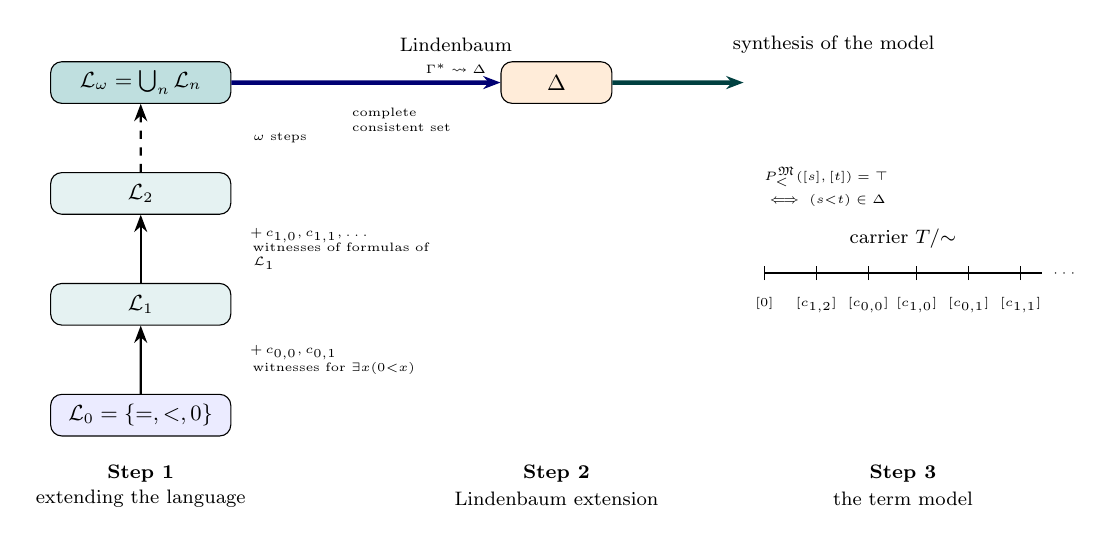
\begin{tikzpicture}[
  scale=0.88, every node/.style={scale=0.88},
  font=\small,
  level/.style={draw, rounded corners, minimum width=2.6cm, minimum height=0.6cm, align=center},
  arrow/.style={-{Stealth[length=2.2mm]}, thick},
  annot/.style={font=\tiny, align=left, text width=2.8cm},
]

% ============ COLUMN 1: language tower ============
\node[level, fill=blue!8]   (L0) at (0,0)   {$\mathcal{L}_0 = \{=,<,0\}$};
\node[level, fill=teal!10]  (L1) at (0,1.6) {$\mathcal{L}_1$};
\node[level, fill=teal!10]  (L2) at (0,3.2) {$\mathcal{L}_2$};
\node[level, fill=teal!25]  (Lw) at (0,4.8) {$\mathcal{L}_\omega = \bigcup_n \mathcal{L}_n$};

\draw[arrow] (L0) -- (L1);
\node[annot, anchor=west] at (1.5,0.8) {$+\,c_{0,0},c_{0,1}$\\witnesses for $\exists x(0{<}x)$};

\draw[arrow] (L1) -- (L2);
\node[annot, anchor=west] at (1.5,2.4) {$+\,c_{1,0},c_{1,1},\ldots$\\witnesses of formulas of $\mathcal{L}_1$};

\draw[arrow, dashed] (L2) -- (Lw);
\node[font=\tiny, anchor=west] at (1.5,4.0) {$\omega$ steps};

\node[font=\footnotesize\bfseries] at (0,-0.85) {Step 1};
\node[font=\footnotesize] at (0,-1.2) {extending the language};

% ============ COLUMN 2: Lindenbaum ============
\node[level, fill=orange!15, minimum width=1.6cm] (Delta) at (6.0,4.8) {$\Delta$};

\draw[arrow, ultra thick, blue!45!black] (Lw) -- (Delta);
\node[font=\footnotesize] at (4.55,5.35) {Lindenbaum};
\node[font=\tiny] at (4.55,5.0) {$\Gamma^* \rightsquigarrow \Delta$};
\node[annot, anchor=north] at (4.45,4.55)
  {complete\\consistent set};

\node[font=\footnotesize\bfseries] at (6.0,-0.85) {Step 2};
\node[font=\footnotesize] at (6.0,-1.2) {Lindenbaum extension};

% ============ COLUMN 3: model carrier ============
\draw[arrow, ultra thick, teal!50!black] (Delta) -- (8.7,4.8);
\node[font=\footnotesize] at (10.0,5.35) {synthesis of the model};

\begin{scope}[shift={(9.0,2.05)}]
\draw[thick] (0,0) -- (4.0,0);
\draw (0,-0.1)    -- (0,0.1);    \node[font=\tiny, below=2pt] at (0,-0.15)    {$[0]$};
\draw (0.75,-0.1) -- (0.75,0.1); \node[font=\tiny, below=2pt] at (0.75,-0.15) {$[c_{1,2}]$};
\draw (1.5,-0.1)  -- (1.5,0.1);  \node[font=\tiny, below=2pt] at (1.5,-0.15)  {$[c_{0,0}]$};
\draw (2.2,-0.1)  -- (2.2,0.1);  \node[font=\tiny, below=2pt] at (2.2,-0.15)  {$[c_{1,0}]$};
\draw (2.95,-0.1) -- (2.95,0.1); \node[font=\tiny, below=2pt] at (2.95,-0.15) {$[c_{0,1}]$};
\draw (3.7,-0.1)  -- (3.7,0.1);  \node[font=\tiny, below=2pt] at (3.7,-0.15)  {$[c_{1,1}]$};
\node[font=\tiny] at (4.35,0) {$\cdots$};
\node[font=\footnotesize] at (2.0,0.5) {carrier $T/{\sim}$};
\end{scope}

\node[annot, anchor=north, text width=4cm] at (11.0,3.7)
  {$P_<^{\mathfrak M}([s],[t])=\top$\\[2pt] $\iff (s{<}t)\in\Delta$};

\node[font=\footnotesize\bfseries] at (11.0,-0.85) {Step 3};
\node[font=\footnotesize] at (11.0,-1.2) {the term model};

\end{tikzpicture}
\end{center}

% ==============================================
\section*{Summary of the Construction}
% ==============================================

\begin{center}
\footnotesize
\begin{tabular}{cp{12cm}}
  \hline
  \textbf{Step} & \textbf{What We Do} \\
  \hline
  1 & Extend the language: add the Henkin constants $c_{n,k}$ iteratively
      (with the witness registry, Remark~\ref{rem:registry}) \\
  2 & Extend $\Gamma$ with the Henkin axioms~--- obtaining $\Gamma^*$,
      consistent by Lemma~\ref{lem:henkin-consistent} \\
  3 & Use the Lindenbaum algorithm to build a CC-set $\Delta \supseteq \Gamma^*$ \\
  4 & The carrier of the model is the set of equivalence classes of closed terms of $\Lw$ \\
  5 & Define the predicates and functions via $\Delta$; well-definedness is given by
      Lemma~\ref{lem:welldefined} (the congruence axioms) \\
  6 & The truth lemma (induction on complexity) gives $\Struct \models \Delta$ \\
  7 & The reduct $\Struct|_{\Lang}$ (Lemma~\ref{lem:reduct}) is a model of the original $\Gamma$ \\
  \hline
\end{tabular}
\end{center}

\vfill
\begin{center}
\rule{0.3\textwidth}{0.4pt}\\[0.5em]
{\footnotesize\color{gray} \copyright\ Nikolai Kazimirov 2026 \quad\textbar\quad \url{https://mathem.at}}
\end{center}

\end{document}
